% !Mode:: "TeX:UTF-8"
\documentclass{article}
% !Mode:: "TeX:UTF-8"
\usepackage[english]{babel}
\usepackage[UTF8]{ctex}
\usepackage{amsmath, amsthm, amssymb}

% Figure
\usepackage{graphicx}
\usepackage{float} %% H can fix the location
\usepackage{caption}
\usepackage[format=hang,singlelinecheck=0,font={sf,small},labelfont=bf]{subfig}
\usepackage[noabbrev]{cleveref}
\captionsetup[subfigure]{subrefformat=simple,labelformat=simple,listofformat=subsimple}
\renewcommand\thesubfigure{(\alph{subfigure})}

\usepackage{epstopdf} %% convert eps to pdf
\DeclareGraphicsExtensions{.eps,.mps,.pdf,.jpg,.png} %% bmp, gif not supported
\DeclareGraphicsRule{*}{eps}{*}{}
\graphicspath{{img/}{figure/}{../figure/}} %% fig directorys

%% \usepackage{pstricks} %% a set of macros that allow the inclusion of PostScript drawings directly inside TeX or LaTeX code
%% \usepackage{wrapfig} %% Wrapping text around figures

% Table
\usepackage{booktabs} %% allow the use of \toprule, \midrule, and \bottomrule
\usepackage{tabularx}
\usepackage{multirow}
\usepackage{colortbl}
\usepackage{longtable}
\usepackage{supertabular}

\usepackage[colorinlistoftodos]{todonotes}

% Geometry
\usepackage[paper=a4paper, top=1.5cm, bottom=1.5cm, left=1cm, right=1cm]{geometry}
%% \usepackage[paper=a4paper, top=2.54cm, bottom=2.54cm, left=3.18cm, right=3.18cm]{geometry} %% ms word
%% \usepackage[top=0.1cm, bottom=0.1cm, left=0.1cm, right=0.1cm, paperwidth=9cm, paperheight=11.7cm]{geometry} %% kindle

% Code
%% \usepackage{alltt} %% \textbf can be used in alltt, but not in verbatim

\usepackage{listings}
\lstset{
    backgroundcolor=\color{white},
    columns=flexible,
    breakatwhitespace=false,
    breaklines=true,
    captionpos=tt,
    frame=single, %% Frame: show a box around, possible values are: none|leftline|topline|bottomline|lines|single|shadowbox
    numbers=left, %% possible values are: left, right, none
    numbersep=5pt,
    showspaces=false,
    showstringspaces=false,
    showtabs=false,
    stepnumber=1, %% interval of lines to display the line number
    rulecolor=\color{black},
    tabsize=2,
    texcl=true,
    title=\lstname,
    escapeinside={\%*}{*)},
    extendedchars=false,
    mathescape=true,
    xleftmargin=3em,
    xrightmargin=3em,
    numberstyle=\color{gray},
    keywordstyle=\color{blue},
    commentstyle=\color{green},
    stringstyle=\color{red},
}

% Reference
%% \bibliographystyle{plain} % reference style

% Color
\usepackage[colorlinks, linkcolor=blue, anchorcolor=red, citecolor=green, CJKbookmarks=true]{hyperref}
\usepackage{color}
\def\red#1{\textcolor[rgb]{1.00,0.00,0.00}{#1}}
\newcommand\warning[1]{\red{#1}}

% Other
%% \usepackage{fixltx2e} %% for use of \textsubscript
%% \usepackage{dirtree}  %% directory structure, like the result of command tree in bash shell

   %导入需要用到的package
% !Mode:: "TeX:UTF-8"
%+++++++++++++++++++++++++++++++++++article+++++++++++++++++++++++++++++++++
%customize the numbering of equation, to make it like section-subsection-equation style, for example,1-2-3
\makeatletter\@addtoreset{equation}{subsection}\makeatother
\renewcommand\theequation{%
\thepart\arabic{section}%
-\thepart\arabic{subsection}%
-\thepart\arabic{equation}%
}
%theorem
\newtheorem{definition}{D\'efintion} %% 整篇文章的全局编号
\newtheorem*{thmwn}{Thm} %% without numbers
\newtheorem{theorem}{Th\'eor\`eme}[section] %% 从属于section编号
\newtheorem{corollary}{Corollary}[theorem] %% 从属于theorem编号
\newtheorem{lemma}{Lemma}
\newtheorem{proposition}{Proposition}[section]
\newtheorem{example}{Example}
\newtheorem*{attention}{Attention}
\newtheorem*{note}{Note}
\newtheorem*{remark}{Remark}
\newtheorem{question}{Question}[section]
\newtheorem{problem}{Problem}
\newtheorem{fact}{Fact}


% Equation
\newcommand\lasteq{(\theequation)\ } %% use \lasteq to reference the last equation
\newcommand{\eqspace}{\hspace{0.5cm}}
\newcommand{\eqnote}[1]{\text{ #1 }} %% insert text in math mode being treated as normal text
\newcommand\mytop[2]{\genfrac{}{}{0pt}{}{#1}{#2}} %% generate a fraction but without the line

% Vecteur
\def\vecteur#1{(#1_1,~#1_2,~\ldots,~#1_n)}
\def\vector#1{#1_1,~#1_2,~\ldots,~#1_n}

% Set
\newcommand{\R}{\mathbb{R}} %% the real number set
\newcommand{\N}{\mathbb{N}}
\newcommand{\Z}{\mathbb{Z}}
\newcommand{\Q}{\mathbb{Q}}
\newcommand{\set}[1]{\{#1\}}
\newcommand{\stcomp}[1]{\overline{#1}} %% set complement

% Logic
\newcommand{\si}{\textrm{\ if }}
\newcommand{\sinon}{\textrm{ si non}}
\newcommand{\then}{\textrm{ then }}
\newcommand{\et}{\textrm{\ et }}
\newcommand{\ou}{\textrm{ ou }}
\newcommand{\non}{\textrm{non }}
\newcommand{\ssi}{si et seulement si }

% Math Operator
\newcommand{\fun}[1]{\textit{#1}}
\DeclareMathOperator{\arccot}{arcot}
\DeclareMathOperator{\arcth}{arcth}
\DeclareMathOperator{\arcsh}{arcsh}
\DeclareMathOperator{\arch}{arch}
\DeclareMathOperator{\ch}{ch}
\DeclareMathOperator{\dth}{th} %% \th already used
\DeclareMathOperator{\sh}{sh}
\DeclareMathOperator{\var}{var}
\DeclareMathOperator{\Ker}{Ker}
\DeclareMathOperator{\Img}{Img}

\newcommand*\laplace{\mathop{}\!\mathbin\bigtriangleup}
\newcommand*\dalambert{\mathop{}\!\mathbin\Box}
\newcommand{\grad}[1]{\nabla #1}
\newcommand{\gradien}[1]{\nabla #1}
\newcommand{\divergence}[1]{\nabla \cdot #1}
\newcommand{\rotationnel}[1]{\nabla \times #1}
\newcommand{\rot}[1]{\nabla \times #1}

\newcommand{\diag}[1]{\textit{diag}(#1)}
\newcommand{\mean}[1]{\overline{#1}}
\newcommand{\estimate}[1]{\hat{#1}}
\newcommand{\indep}{\!\perp\!\!\!\perp}
\newcommand{\nindep}{\not\!\perp\!\!\!\perp}
\newcommand{\norm}[1]{\left\Vert #1\right\Vert}
\newcommand{\obey}[1]{\thicksim{#1}}

\usepackage{xspace}
\newcommand{\ps}[2]{\ensuremath{\langle #1 , #2\rangle}\xspace} %% produit scalaire

%% quantique operators
\newcommand\ket[1]{|#1\rangle}
\newcommand\bra[1]{\langle #1|}
\newcommand\braket[3]{\langle#1|#2|#3\rangle}

% Symbol
\newcommand{\infinity}{\infty}


\begin{document}
\title{Mes Notes d'Variation}
\author{Eric}
\maketitle
\tableofcontents
\newpage

\section{Fundamental lemma of variation}
\begin{theorem}
    Soit une fonction $f(x)$ est continue sur $[a,b]$,$ \forall \eta(x)$ sur $\in C^{n}[a,b]$,et $\exists m>0$,tel que $\eta^{k}(a)=\eta^{k}(b)=0 (\forall k \in [[0,n]])$ \newline
    si$ \int_{a}^{b}f(x)\eta(x)=0$ est toujours vrai, \newline
    alors, sur $[a,b],f(x)\equiv 0$ \newline
    (证明时用反证法,且需要构造$\eta(x)$为特殊的形式)
    $\exists \xi,f(\xi)>0 \Rightarrow \exists $une intervale $[a_0,b_0]$,tel que sur $[a_0,b_0],f(x)$ est positive \newline
 on peut construire $\eta(x)$ comme cidessous:
$\eta(x)=
    \left\{
      \begin{array}{ll}
        [(x-a_0)(x-b_0)]^{2n+2} & x \in [a_0,b_0] \\
        0 & sinon
      \end{array}
    \right.
    $
\end{theorem}

\textbf{Quand m=n=0}
\begin{theorem}
    Soit une fonction $f(x)$ est continue sur $[a,b]$,$ \forall \eta(x)$ sur $\in C^{0}[a,b]$,et $\exists m>0$,tel que $\eta(a)=\eta(b)=0$ \newline
    si$ \int_{a}^{b}f(x)\eta(x)=0$ est toujours vrai, \newline
    alors, sur $[a,b],f(x)\equiv 0$
\end{theorem}

\begin{theorem}
    Soit une fonction $f(x)$ est continue sur $[a,b]$,$ \forall \eta(x)$ sur $\in C^{1}[a,b]$,et $\eta(a)=\eta(b)=0$ \newline
    si$ \int_{a}^{b}f(x)\eta'(x)=0$ est toujours vrai, \newline
    alors, sur $[a,b],f(x)\equiv Constante$
\end{theorem}

\begin{theorem}
    Soit une fonction $f(x,y)$ est continue sur $D$,$ \forall \eta(x,y)$ sur $\in C^{1}[a,b]$,et 在D的边界上, $\eta(x,y)=0$\newline
    si$ \int_{a}^{b}f(x,y)\eta(x,y)=0$ est toujours vrai, \newline
    alors, sur $D,f(x,y)\equiv 0$
\end{theorem}

\section{Variational Problems with Fixed Boudaries}
\begin{definition}
  \textbf{n阶距离}:Soit deux foncitons $y(x)$ et $y_0(x)\in C^{n}[a,b]$,则这两个函数从0到n阶导数之差的绝对值中的最大值称为 $y(x)$ et $y_0(x)$在区间$[a,b]$上的n阶距离或n级距离
  $d_n[y(x),y_0(x)]=max_{0 \leqslant i \leqslant n}max_{a \leqslant x \leqslant b}|y^{(i)}(x)-y_0^{(i)}(x)|$
\end{definition}
特别地,当$n=0$时,为0阶距离;当$n=1$时,为1阶距离

\begin{definition}
\textbf{n阶领域}:函数$y_0(x)$在区间$[a,b]$上的n阶领域,记为$N_n[\delta,y_0(x)]$,表示为\newline
$N_n[\delta,y_0(x)]=\{y(x)|y(x)\in C^{n}[a,b],d_n[y(x),y_0(x)] < \delta \}$
\end{definition}
\begin{definition}
\textbf{变分}:对于任意定值$x \in [x_0,x_1]$,可取函数$y(x)$ 与另一个可取函数 $y_0(x)$ 之差$y(x)-y_0(x)$ 称为函数$y(x)$在 $y_0(x)$ 处的变分或函数的变分,记作$\delta y$,$\delta$称作变分符号或变分算子,这时有\\
$\delta y=y(x)-y_0(x)=\epsilon\eta(x)$ \newline
式中$\epsilon$为朗格朗日引进的一个小参数,但是不是x的函数,而$\eta(x)$为x的任意函数
\end{definition}
由于可取函数都通过区间的固定端点,即他们在区间的端点的值相等,且由于端点是固定的,所以在端点处的变分为零. \newline

可取函数$y(x)$ 是泛函$J[y(x)]$的宗量,故也可以这样定义变分:泛函的宗量$y(x)$与另一个宗量 $y_0(x)$ 之差$y(x)-y_0(x)$ 称为宗量$y(x)$在 $y_0(x)$ 处的变分.

\begin{attention}
函数的变分$\delta y$是x的函数.\newline
注意函数变分与函数增量$\Delta y$的区别:\newline
函数的变分是两个不同函数在x取一个定值时之差,函数发生了改变,自变量没有变;\newline
而函数的增量是由于自变量x取一个增量而使同一个函数产生的增量,函数仍是原来的函数,而自变量发生了变化
\end{attention}

\textbf{全变分}:若可取函数$y(x)$变位$y_1(x)$的同时,自变量x也取得了无穷小增量$\Delta x$,函数的增量在舍去高阶增量后,可近似写成\newline
$\Delta y=\delta y + y'(x)\Delta x$
\newline
全变分包括两部分,一部分是由于自变量变化所引起的$y'(x)\Delta x$;另一部分是由函数变化所引起的$\delta y $

$\delta y'=y'(x)-y_0'(x)=[y(x)-y_0(x)]'=(\delta y)'$
D'ou $\delta \frac{dy}{dx}=\frac{d}{dx}\delta y$
\newline
That is to say:函数导数的变分等于函数变分的倒数,换句话说,求变分与求导数这两种运算次序可以交换
\newline
上面的性质可以推广到高阶的情形
同时,我们可以推出哈密顿算子,拉普拉斯算子都可以和变分符号交换顺序

\subsection{最简泛函的变分与极值的必要条件}
Soit $F(x,y(x),y'(x))$ une fonction connue de trois variables $x,y(x),y'(x)$ sur $[x_0,x_1]$, et F 二阶连续可微,其中$y(x),y'(x)$是x的未知函数,则泛函 \newline
$$J[y(x)]=\int_{x_0}^{x_1}F(x,y(x),y'(x))dx$$
称为最简单的积分型泛函,简称最简泛函,$J[y(x)]$ 是$y(x)$的泛函,由上面的式子知,$J[y(x)]$不仅是$y(x)$的函数,而且还是$x,y'(x)$, 但是只要求出了$y(x)$, $y'(x)$也就能够求出来了, 于是泛函只是写成$J[y(x)]$的形式
\newline
最简泛函的增量也称为泛函的全变分
\begin{equation}
\begin{split}
  \Delta J=J[y_1(x)]-J[y(x)]=J[y(x)+\delta y]-J[y(x)]= \\
\int_{x_0}^{x_1}F(x,y(x)+\delta y,y'(x)+\delta y')dx-\int_{x_0}^{x_1}F(x,y(x),y'(x))dx = \\
\int_{x_0}^{x_1}[F(x,y(x)+\delta y,y'(x)+\delta y')-F(x,y(x),y'(x))]dx
 \end{split}
\end{equation}
$F(x,y(x)+\delta y,y'(x)+\delta y')-F(x,y(x),y'(x))=\overline{F_y}\delta y + \overline{F_{y'}}\delta y'$ \newline
$F(x,y(x)+\delta y,y'(x)+\delta y')-F(x,y(x),y'(x))$的线性部分是$F_y\delta y + F_{y'}\delta y'$ \\
On note $F_y\delta y + F_{y'}\delta y'$ comme $L[y,\delta y]$ \\
$L[y,\delta y]$ 是关于$\delta y$的现行泛函

\begin{definition}
若连续泛函$J[y(x)]$满足以下两个条件:\\
1. $J[y_1(x)+y_2(x)]=J[y_1(x)]+J[y_2(x)]$ \\
2. $J[cy(x)]=cJ[y(x)]$ avec c une constante\\
alors,$J[y(x)]$称为关于$y(x)$的线性泛函
\end{definition}

对称双线性泛函,双线性泛函,二次泛函\\
$$
\delta J
=\int_{x_0}^{x_1}[F_y(x,y,y')\delta y + F_{y'}(x,y,y')\delta y']dx
=\int_{x_0}^{x_1}(F_y\delta y + F_{y'}\delta y')dx
=\int_{x_0}^{x_1}(F_y\epsilon\eta + F_{y'}\epsilon\eta')dx
=\epsilon \int_{x_0}^{x_1}(F_y\eta + F_{y'}\eta')dx
$$
泛函的变分$\delta J$是泛函增量$\Delta J$的线性主要部分,即线性主部

变分记号$\delta$有下列基本运算性质\\
1.$\delta (F_1+F_2)=\delta F_1+\delta F_2$ \\
2.$\delta (F_1*F_2)=F_1\delta F_2+F_2\delta F_1$\\
3.$\delta (F^{n})=nF^{n-1}\delta F$\\
4.$\delta (\frac{F_1}{F_2})=\frac{F_2\delta F_1-F_1\delta F_2}{F_2^{2}}$\\
5.$\delta (F^{(n)})=(\delta F)^{n}$\\
6.$\delta \int_{x_0}^{x_1}F(x,y,y')dx=\int_{x_0}^{x_1}\delta F(x,y,y')dx$\\

全变分$\Delta$有下列基本运算性质\\
1.$\Delta (F_1+F_2)=\Delta F_1+\Delta F_2$ \\
2.$\Delta (F_1*F_2)=F_1\Delta F_2+F_2\Delta F_1$\\
3.$\Delta (F^{n})=nF^{n-1}\Delta F$\\
4.$\Delta (\frac{F_1}{F_2})=\frac{F_2\Delta F_1-F_1\Delta F_2}{F_2^{2}}$\\
5.$(\Delta F^{(n)})'=\Delta( F^{(n+1)})+F^{(n+1)}(\Delta x)'$ (微分与全变分的运算次序不能交换)\\
6.$\Delta \int_{x_0}^{x_1}Fdx=\delta \int_{x_0}^{x_1}Fdx + (F\delta x)|_{x_0}^{x_1}=\int_{x_0}^{x_1}(\delta F + F\frac{d}{dx}\delta x)dx $  \\性质6表明,当$\frac{d}{dx}\delta x\neq 0$时,积分与全变分的运算也不能交换顺序 \\
7.$d(\Delta x) = \Delta(dx)$
对自变量而言,全变分和微分的运算次序具有交换性

5.preuve: \\
$(\Delta F^{(n)})'=[F^{(n+1)} \Delta x + \delta (F^{(n)})]'=F^{(n+2)}\Delta x + F^{(n+1)}(\Delta x)'+ \delta (F^{(n+1)})=\Delta (F^{(n+1)}) + F^{(n+1)}(\Delta x)'$

6.preuve: \\
$$\Delta \int_{0}^{x}Fdx=\delta \int_{0}^{x}Fdx + F \Delta x$$
将上式中的积分上限x分别用$x_0,x_1$替换,可得到两个类似的关系式,然后将两个式子作差,可得到下面的关系式:
$$\Delta \int_{x_0}^{x_1}Fdx=\delta \int_{x_0}^{x_1}Fdx + (F \Delta x)|_{x_0}^{x_1}$$
and
$$\delta \int_{x_0}^{x_1}Fdx=\int_{x_0}^{x_1}\delta Fdx=\int_{x_0}^{x_1}(\Delta F -F' \Delta x)dx $$
$$(F \Delta x)|_{x_0}^{x_1}=\int_{x_0}^{x_1}d(F \Delta x)$$
将上面的两个式子代入到上面的第三个式子中得到:
$$\Delta \int_{0}^{x}Fdx=\int_{x_0}^{x_1}(\Delta F -F' \Delta x)dx +\int_{x_0}^{x_1}d(F \Delta x)=\int_{x_0}^{x_1}[\Delta F + F (\Delta x)']dx$$
\subsection{最简泛函的欧拉方程}
\begin{theorem}
使最简泛函
$$J[y(x)]=\int_{x_0}^{x_1}F(x,y(x),y'(x))dx$$
取极值且满足固定边界条件
$$
y(x_0)=y_0,y(x_1)=y_1
$$
的极值曲线$y=y(x)$应满足\textbf{必要条件}(欧拉方程)
$$
F_y - \frac{d}{dx}F_{y'} =0
$$
的解,式中$F$是$x,y,y'$的已知函数并有二阶连续偏导数
取得极值 $\Leftrightarrow \delta J = \int_{x_0}^{x_1}(F_y \delta y + F_{y'} \delta y')dx=0$
\end{theorem}

\subsection{依赖于多个一元函数的变分问题}
\begin{theorem}
使泛函$$J[y(x),z(x)]=\int_{x_0}^{x_1}F(x,y,y',z,z')dx$$取得极值且满足固定边界条件
$$
y(x_0)=y_0,y(x_1)=y_1,z(x_0)=z_0,z(x_1)=z_1
$$
的极值曲线$y=y(x),z=z(x)$必满足欧拉方程组
$$
\left\{
  \begin{array}{ll}
    F_y - \frac{d}{dx}F_{y'}=0 & \\
    F_z - \frac{d}{dx}F_{z'}=0 &
  \end{array}
\right.
$$
\end{theorem}

\begin{corollary}
对于含有n个未知数$y_1(x),y_2(x) ,\ldots , y_n(x)$,使泛函
$$J[y_1,y_2 ,\ldots , y_n]=\int_{x_0}^{x_1}F(x,y_1,y_2 ,\ldots , y_n,y_1',y_2' ,\ldots , y_n')dx$$
取得极值并且满足边界条件
$$y_i(x_0)=y_{i0},y_i(x_1)=y_{i1} ~(i=1,2,\dots,n)$$
的极值曲线$y_i=y_i(x)~ (i=1,2,\dots,n)$比满足欧拉方程组
$$F_{y_i} -  \frac{d}{dx}F_{y_i'}=0 ~(i=1,2,\dots,n)$$
\end{corollary}

\subsection{依赖于高阶导数的变分问题}
\begin{theorem}
使泛函
$$J[y(x)]=\int_{x_0}^{x_1}F(x,y,y',y'')dx$$
取极值且满足固定边界条件
$$
y(x_0)=y_0,y(x_1)=y_1,y'(x_0)=y_0',y'(x_1)=y_1'
$$
的极值曲线$y=y(x)$必满足微分方程
$$F_y - \frac{d}{dx}F_y' + \frac{d^2}{dx^2}F_{y''} = 0 $$
\end{theorem}

\begin{corollary}
使依赖于未知函数$y(x)$的n阶导数的泛函
$$J[y]=\int_{x_0}^{x_1}F(x,y,y',y'', \ldots , y^{(n)})dx$$
取极值且满足固定边界条件
$$
y^{(k)}(x_0)=y_0^{(k)}, y^{(k)}(x_1)=y_1^{(k)} ~ (k= 0,1,\ldots , n-1)
$$
的极值曲线$y=y(x)$必满足欧拉-泊松方程
$$F_y - \frac{d}{dx}F_{y'} + \frac{d^2}{dx^2}F_{y''} - \dots + (-1)^{n}\frac{d^n}{dx^n}F_{y^{(n)}}=0  $$
式中F具有n+1阶连续导数,y具有2n阶连续导数,这是一个2n阶微分方程,它的通解中含有2n个特定常数,可由2n个边界来确定
\end{corollary}

\begin{corollary}
使依赖于两个未知函数$y(x)$的m阶导数,$z(x)$的n阶导数的泛函
$$J[y(x),z(x)]=\int_{x_0}^{x_1}F(x,y,y',y'', \ldots , y^{(m)},z,z',z'', \ldots , z^{(n)})dx$$
取极值且满足固定边界条件
$$
y^{(k)}(x_0)=y_0^{(k)}, y^{(k)}(x_1)=y_1^{(k)} ~ (k= 0,1,\ldots , m-1)
$$
$$
z^{(k)}(x_0)=z_0^{(k)}, z^{(k)}(x_1)=z_1^{(k)} ~ (k= 0,1,\ldots , n-1)
$$
的极值曲线$y=y(x),z=z(x)$必满足欧拉-泊松方程
$$
\left\{
  \begin{array}{ll}
    F_y - \frac{d}{dx}F_{y'} + \frac{d^2}{dx^2}F_{y''} - \dots + (-1)^{n}\frac{d^n}{dx^n}F_{y^{(n)}}=0 &\\
    F_z - \frac{d}{dx}F_{z'} + \frac{d^2}{dx^2}F_{z''} - \dots + (-1)^{n}\frac{d^n}{dx^n}F_{z^{(n)}}=0   &
  \end{array}
\right.
$$
式中F具有n+1阶连续导数,y,z具有2n阶连续导数
\\
当然我们还可以推论到更多个未知函数的情况
\end{corollary}

\subsection{依赖于多元函数的变分问题}
\begin{theorem}
设D是平面区域,$(x,y) \in D ,u(x,y) \in C^2(D)$,使泛函
$$
J[u(x,y)]=\int\int_{D}F(x,y,u_x,u_y)dxdy
$$
取极值且在区域D的边界线L上取已知的极值函数$u=u(x,y)$必须满足偏微分方程
$$
F_u -\frac{\partial}{\partial x}F_{u_x}-\frac{\partial}{\partial y}F_{u_y} = 0
$$
这个方程称为奥斯特罗格拉茨基方程,简称奥氏方程,有时也称之为欧拉方程
\end{theorem}

\begin{corollary}
设D是平面区域,$(x,y) \in D ,u(x,y) \in C^4(D),F(x,y,u,u_x,u_y,u_{xx},u_{xy},u_{yy}) \in C^3$,则泛函
$$
J[u(x,y)]=\int\int_{D}F(x,y,u,u_x,u_y,u_{xx},u_{xy},u_{yy})dxdy
$$
的奥氏方程为
$$
F_u -\frac{\partial}{\partial x}F_{u_x}-\frac{\partial}{\partial y}F_{u_y}+ \frac{\partial^2}{\partial x^2}F_{u_{xx}} + \frac{\partial^2}{\partial x \partial y}F_{u_{xy}} + \frac{\partial^2}{\partial y^2}F_{u_{yy}} = 0
$$
\end{corollary}

\begin{corollary}
设D是平面区域,$(x,y) \in D, u(x,y) \in C^{2n}(D),F \in C^{n+1}(D)$,则泛函
$$
J[u(x,y)]=\int\int_{D}F(x,t,u,u_x,u_y,u_{xx},u_{yy}, \ldots , u_{\underbrace{xx \dots x}_{n}},u_{\underbrace{yy \dots y}_{n}})dxdy
$$
的奥氏方程为
$$
\begin{array}{c}
   F_u -\frac{\partial}{\partial x}F_{u_x}-\frac{\partial}{\partial y}F_{u_y}+ \frac{\partial^2}{\partial x^2}F_{u_{xx}} + \frac{\partial^2}{\partial x \partial y}F_{u_{xy}} + \frac{\partial^2}{\partial y^2}F_{u_{yy}} + \dots +  \\
 \\
   (-1)^n (
\frac{\partial^n }{\partial x^n}F_{u_{\underbrace{xx \dots x}_{n}}}+
\frac{\partial^n }{\partial x^{n-1}\partial y}F_{u_{\underbrace{xx \dots y}_{n-1}}}+
\dots+
\frac{\partial^n }{\partial y^n}F_{u_{\underbrace{yy \dots y}_{n}}})
= 0
\end{array}
$$
\end{corollary}

\begin{corollary}
设D是平面区域,$(x,y) \in D ,u(x,y) \in C^2(D),v(x,y) \in C^2(D)$,使泛函
$$
J[u(x,y),v(x,y)]=\int\int_{D}F(x,y,,u,v,u_x,,v_x,u_y,v_y)dxdy
$$
的奥氏方程组为
$$
\left\{
  \begin{array}{ll}
   F_u -\frac{\partial}{\partial x}F_{u_x}-\frac{\partial}{\partial y}F_{u_y} = 0 \\
   F_v -\frac{\partial}{\partial x}F_{v_x}-\frac{\partial}{\partial y}F_{v_y} = 0
  \end{array}
\right.
$$
\end{corollary}

\section{可动边界的变分问题}
\subsection{最简泛函的变分问题}
设泛函
\begin{equation}
  J[y(x)]=\int_{x_0}^{x_1}F(x,y,y')dx
\label{equation.function.simple-general}
\end{equation}

其可取曲线$y = y(x) \in C^2$类函数,且两个端点$A(x_0,y_0),B(x_1,y_1)$ 分别在两个给定的$C^2$类函数,此时称为可动边界的最简泛函或待定边界的最简泛函。\\

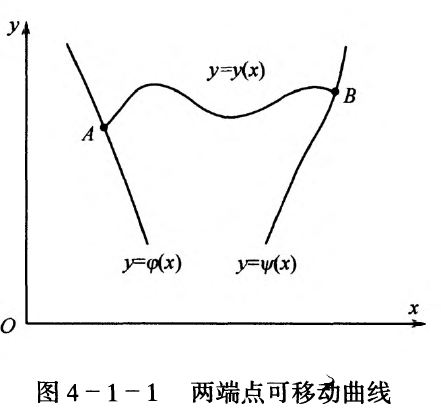
\includegraphics[width=0.5\textwidth]{image/limit-move}\\

若函数$y=y(x)$能在可动边界的容许函数类中使泛函(\ref{equation.function.simple-general})取得极值,
那么必能在固定边界的容许函数类中使泛函取得极值,这是因为可动边界泛函的容许曲线类的范围扩大了,当然包含了固定边界泛函的容许曲线,
而在固定边界情况下使泛函取得极值的函数必须满足欧拉方程,所以函数(\ref{equation.function.simple-general})在可动边界情况下也应当满足欧拉方程
$$
F_y - \frac{d}{dx}F_{y'} =0
$$
欧拉方程的解含有两个任意常数,它的一般解形式为
$$y=y(x,c_1,c_2)$$
在端点固定的情况下,这两个常数可以解出来,在可动边界条件下,他们都是$x_0,x_1$的函数,确定他们的条件就是泛函取得极值的必要条件$\delta J=0$

如图所示,A点固定,B点可以变动,当B点从$(x_1,y_1)$移动到$(x_1+\delta x_1,y_1+\delta y_1)$时,泛函$ J[y(x)]$的增量
\begin{equation}
     \begin{split}
         & \Delta J=\int_{x_0}^{x_1+\delta x_1}F(x,y+\delta y,y'+\delta y')dx-\int_{x_0}^{x_1}F(x,y,y')dx\\
         & =\int_{x_0}^{x_1+\delta x_1}F(x,y+\delta y,y'+\delta y')dx+\int_{x_0}^{x_1}[F(x,y+\delta y,y'+\delta y')-F(x,y,y')]dx
     \end{split}
\end{equation}
略去高阶无穷小量后剩下一阶变分为
\begin{equation}
\begin{split}
     &  \delta J=\int_{x_0}^{x_1}(F_y - \frac{d}{dx}F_{y'} )\delta y dx + F|_{x=x_1}\delta x_1 + F_{y'}|_{x=x_1}[\delta y_1 - y'(x_1)\delta x_1] \\
    & =\int_{x_0}^{x_1}(F_y - \frac{d}{dx}F_{y'} )\delta y dx + (F-y'F_{y'})|_{x=x_1}\delta x_1 +F_{y'}|_{x=x_1}\delta y_1
\end{split}
\end{equation}
因为泛函的极值只能在极值曲线上取得,所以
$F_y - \frac{d}{dx}F_{y'} \equiv0$
上式化为
\begin{equation}
     \delta J=(F-y'F_{y'})|_{x=x_1}\delta x_1 +F_{y'}|_{x=x_1}\delta y_1
\end{equation}
再由条件$\delta J=0$得
\begin{equation}
     (F-y'F_{y'})|_{x=x_1}\delta x_1 +F_{y'}|_{x=x_1}\delta y_1=0
     \label{equation.result.general}
\end{equation}
如果$\delta x_1,\delta y_1$相互无关,则由(\ref{equation.result.general})得到
\begin{equation}
(F-y'F_{y'})|_{x=x_1}=0
\label{equation.result.unrelated.1}
\end{equation}
\begin{equation}
F_{y'}=0
\label{equation.result.unrelated.2}
\end{equation}
当我们把(\ref{equation.result.unrelated.2})代入(\ref{equation.result.unrelated.1})我们得到$F_y=0$,因此我们有必要考虑$\delta x_1,\delta y_1$相关
\begin{theorem}
设泛函$J[y(x)]=\int_{x_0}^{x_1}F(x,y,y')dx$的极值曲线$y=y(x)$一端固定,另一端在直线$x=x_1$上待定,则可动的一端必满足自然边界条件(\ref{equation.result.unrelated.2})
若极值曲线$y=y(x)$的端点在已知直线$y=\psi(x)$上待定,则变分$\delta x_1,\delta y_1$相关
\end{theorem}

\begin{theorem}
设泛函$J[y(x)]=\int_{x_0}^{x_1}F(x,y,y')dx$的极值曲线$y=y(x)$左端固定,右端点在已知直线$y=\psi(x)$上待定,则右端点在$x=x_1$处必满足
\begin{equation}
[F + (\psi' - y')F_{y'}]|_{x=x_1}=0
\end{equation}
\end{theorem}
\begin{proof}
 对已知曲线$y=\psi(x)$取变分,得到 $\delta y=\psi'(x)\delta x$,在右端点处,$\delta y_1=\psi'(x_1)\delta x_1$ \\
将之代入到(\ref{equation.result.general})可以得到
$$
[F + (\psi' - y')F_{y'}]|_{x=x_1}\delta x_1=0
$$
又因为$\delta x_1$是任意的,所以可以得到
$[F + (\psi' - y')F_{y'}]|_{x=x_1}=0$
\end{proof}
上式建立了极值曲线$y = y ( x )$与已知曲线:$y = \psi(x)$在交点B 处的$y'$与$\psi'$两斜率
之间的关系,这样的关系称为横截(性)条件、贯截条件或斜截条件。这两条曲线较小的那个交角称
为斜截角。

\begin{theorem}
\label{theorem.limit.two}
设泛函$J[y(x)]=\int_{x_0}^{x_1}F(x,y,y')dx$的极值曲线$y=y(x)$左端固定在直线$y=\varphi(x)$,右端点在已知直线$y=\psi(x)$上待定,\\
则左端点在$x=x_0$处必满足
\begin{equation}
[F + (\varphi' - y')F_{y'}]|_{x=x_0}=0
\end{equation}
则右端点在$x=x_1$处必满足
\begin{equation}
[F + (\psi' - y')F_{y'}]|_{x=x_1}=0
\end{equation}
\end{theorem}
求平面上两条曲线的最短距离是定理(\ref{theorem.limit.two})的一个常见的应用,在此情况下,该定理可以化为更具体的形式.该问题归结为求泛函
$$J[y]=\int_{x_0}^{x_1}\sqrt{1+y'^2}dx$$的极小值

\subsection{含有多个函数的泛函的变分问题}
设空间曲线
\begin{equation}
J[y(x),z(x)]=\int_{x_0}^{x_1}F(x,y,z,y',z')dx
\label{equation.general.space}
\end{equation}
式中$y,z \in C^2[x_0,x_1],F \in C^2$,容许曲线$y=y(x),z=z(x)$在左端点
$A(x_0,y_0,z_0)$固定,右端点 $B(x_1,y_1,z_1)$待定
泛函的(\ref{equation.general.space})的变分可模仿上节的方法进行
\begin{equation}
\begin{array}{c}
  \Delta J=\int_{x_0}^{x_1+\delta x_1}F(x,y+\delta y,z+\delta z,y'+\delta y',z'+\delta z')dx-\int_{x_0}^{x_1}F(x,y,z,y',z')dx\\
\\
  = \int_{x_1}^{x_1+\delta x_1}F(x,y+\delta y,z+\delta z,y'+\delta y',z'+\delta z')dx +\\
\\
\int_{x_0}^{x_1}[F(x,y+\delta y,z+\delta z,y'+\delta y',z'+\delta z')-F(x,y,z,y',z')]dx
\end{array}
\end{equation}
它的线性主部
\begin{equation}
 \delta J=F|_{x=x_1}\delta x_1 +F_{y'}\delta y|_{x=x_1} +F_{z'}\delta z|_{x=x_1} +
 \int_{x_0}^{x_1}[(F_y - \frac{d}{dx}F_{y'}) \delta y +(F_z -\frac{d}{dx}F_{z'} )\delta z]dx
\end{equation}
因为泛函$J[y,z]$的极值只能在极值曲线上取得,故必须满足欧拉方程组
$$
\left\{
  \begin{array}{ll}
    F_y - \frac{d}{dx}F_{y'}=0 & \\
    F_z - \frac{d}{dx}F_{z'}=0 &
  \end{array}
\right.
$$
这个方程组的通解中含有四个任意常数,由于B点可以变动,又多了一个未知量$x_1$,为了使泛函(\ref{equation.general.space})有唯一一组解,就需要确定五个常数.因为A点固定,由$y(x_0)=y_0,z(x_0)=z_0$可以定出两个常数,其余三个常数可根据泛函的极值条件$\delta J=0$确定
将欧拉方程组代入得到
\begin{equation}
 \delta J=F|_{x=x_1}\delta x_1 +F_{y'}\delta y|_{x=x_1} +F_{z'}\delta z|_{x=x_1}=0
\end{equation}
根据上一节的讨论有
\begin{equation}
 \delta y|_{x=x_1}=\delta y_1 - y'(x_1)\delta x_1, \delta z|_{x=x_1}=\delta z_1 - z'(x_1)\delta x_1
\end{equation}
代入上式得
\begin{equation}
 \delta J=(F - y'F_{y'} - z'F_{z'})|_{x=x_1} + F_{y'}|_{x=x_1}\delta y_1 + F_{z'}|_{x=x_1}\delta z_1=0
\label{equation.cases}
\end{equation}
式中的$\delta x_1.\delta y_1,\delta z_1$是任意的,即B点可以按照任意方式变动.根据$y_1,z_1与x_1$之间的关系,可分四种情况来讨论
\\
(1)若变分$\delta x_1.\delta y_1,\delta z_1$相互无关,则可以得到
$$
\left\{
  \begin{array}{ll}
     & (F - y'F_{y'} - z'F_{z'})|_{x=x_1}=0 \\
     &  F_{y'}|_{x=x_1}=0\\
     & F_{z'}|_{x=x_1}=0
  \end{array}
\right.
$$
此时,如果把后两式代入第一个式子中,则有$F|_{x=x_1}=0$,即泛函的被积函数为零,一般来说这样的变分问题无意义
\\
(2)若边界点$B(x_1,y_1,z_1)$沿着某一曲线
$y_1=\varphi(x_1),z_1=\psi(x_1)$
变动时,则
$\delta y_1=\varphi'(x_1)\delta x_1,\delta z_1=\psi'(x_1)\delta x_1$
将他们代入(\ref{equation.cases})并整理,同时注意到$\delta x_1$是任意的,得
\begin{equation}
 [F + (\varphi' - y')F_{y'} + (\psi' -z')F_{z'}]|_{x=x_1}=0
\label{equation.case2}
\end{equation}
式(\ref{equation.case2})称为泛函$J[y,z]$的极值曲线与端点曲线及极值问题的横截条件,它与方程
$y_1=\varphi(x_1),z_1=\phi(x_1)$
一起就能确定欧拉方程组的通解中的任意常数
\\
(3)若边界点$B(x_1,y_1,z_1)$沿着某一曲面$\phi(x_1,y_1,z_1)=0$变动,则
\begin{equation}
 \phi_{x_1}\delta x_1+
 \phi_{y_1}\delta y_1+
 \phi_{z_1}\delta z_1=0
\end{equation}
设$\phi_{x_1}\neq 0$,则可解出$\delta z_1$
代入(\ref{equation.cases})得
\begin{equation}
(F - y'F_{y'} - z'F_{z'} - F_{z'}\frac{\phi_x}{\phi_z})|_{x=x_1} \delta x_1 +
(F_{z'} -F_{z'}\frac{\phi_y}{\phi_z})|_{x=x_1} \delta y_1  )
=0
\end{equation}
由于$\delta x_1,\delta y_1$是任意的,故边界条件为
\begin{equation}
\left\{
  \begin{array}{lll}
     & (F - y'F_{y'} - z'F_{z'} - F_{z'}\frac{\phi_x}{\phi_z})|_{x=x_1} =0 \\
&\\
    & (F_{z'} -F_{z'}\frac{\phi_y}{\phi_z})|_{x=x_1} =0
  \end{array}
\right.
\label{equation.case3}
\end{equation}
将(\ref{equation.case3})与曲面方程$\phi(x_1,y_1,z_1)=0$联立,即可求出极值曲线
\\
(4)若边界点$B(x_1,y_1,z_1)$可在空间平面$x=x_1$上变动,则$\delta x_1=0$,$\delta y_1,\delta z_1$可任意取值,自然边界条件为
\begin{equation}
F_{y'}|_{x=x_1}=0,
F_{z'}|_{x=x_1}=0
\end{equation}

\subsection{含有高阶导数的泛函的变分问题}
设泛函
\begin{equation}
 J[y(x)]=\int_{x_0}^{x_1}F(x,y,y',y'')dx
\end{equation}
式中$y \in C^2[x_0,x_1],F \in C^3$,容许曲线$y=y(x)$在左端点$A(x_0,y_0)$固定,在右端点$B(x_1,y_1)$可变,泛函的极值曲线必满足欧拉-泊松方程
$$F_y - \frac{d}{dx}F_{y'} + \frac{d^2}{dx^2}F_{y''}=0  $$
通常情况下,上式是一个四阶微分方程,其通解含有四个任意常数,右端点B可变,所以$x_1$也待定,总共五个任意常数,左端点A固定可以确定两个,
剩余的三个任意常数必须通过泛函取得极值的必要条件$\delta J=0$得到
这里还是就一般情况进行讨论,先计算泛函的增量$\Delta J$,然后再分离出线性主部$\delta J$
泛函的增量
\begin{equation}
 \begin{split}
 \Delta J = & \int_{x_0}^{x_1+\delta x_1}F(x,y+\delta y,y'+\delta y',y''+\delta y'')dx- \int_{x_0}^{x_1}F(x,y,y',y'')dx \\
              &  =\int_{x_1}^{x_1+\delta x_1}F(x,y+\delta y,y'+\delta y',y''+\delta y'')dx + \\
               & \int_{x_0}^{x_1}[F(x,y+\delta y,y'+\delta y',y''+\delta y'') -F(x,y,y',y'') ]dx
 \end{split}
\end{equation}
最后化简得
\begin{equation}
\begin{split}
 \delta J = & [F - y'(F_{y'}-\frac{d}{dx}F_{y''}) - y''F_{y''}]|_{x=x_1} \delta x_1 + \\
 & (F_{y'}-\frac{d}{dx}F_{y''})|_{x=x_1}\delta y_1 + F_{y''}\delta y_1 =0
\end{split}
\end{equation}
如果上式中$\delta x , \delta y_1, \delta y'_1$之间是相互独立的,则他们的系数在点$x=x_1$处应该为零,及自然边界条件
\begin{equation}
\left\{
  \begin{array}{ll}
[F - y'(F_{y'}-\frac{d}{dx}F_{y''}) - y''F_{y''}]|_{x=x_1}=0 \\
(F_{y'}-\frac{d}{dx}F_{y''})|_{x=x_1}=0\\
F_{y''}=0
  \end{array}
\right.
\end{equation}
同样,若把后两式代入第一式中,仍可得到$F|_{x=x_1}=0$,一般情况下,这样的变分问题无意义.若使变分问题有意义,应在可动的右端点给出一个已知条件。于
是,三个式子中的后两个条件、右端点给出的一个已知条件加上固定端点的两个条件,就可以确 定极值曲线
$y=y(x,c_1,c_2,c_3,c_4)$中的五个待定常量
中的五个待定常量。
\begin{theorem}
 高阶泛函在某一端点固定$y(x_0)=y_0,y'(x_0)=y'_0$,另一端点$(x_1,y_1)$在给定一个已知条件下,其极值曲线$y=y(x)$在端点处
必满足自然边界条件的后两个条件
\end{theorem}

\subsection{单侧变分问题}
如果变分问题中的极值函数服从于某个不等式,则把受有这种不等式约束的变分问题成为单侧变分问题.考虑最简泛函
\begin{equation}
 J[y(x)]=\int_{x_0}^{x_1}F(x,y,y')dx
\end{equation}
在不等式
\begin{equation}
 y(x) \geqslant \varphi(x)
\end{equation}
约束条件下的极值条件,其中$\varphi(x)$是给定的具有连续倒数的函数
\begin{theorem}
 极值曲线$y=y(x)$与曲线$y=\varphi(x)$在M,N两点相切
\end{theorem}

\section{条件极值的变分问题}
\subsection{完整约束的变分问题}
本节主要研究
\begin{equation}
J[y]=\int_{x_0}^{x_1}F(x,y_1,y_2, \cdots , y_n,y_1',y_2', \cdots , y_n')dx
\label{equation.fonctionGenerale}
\end{equation}
在约束条件
\begin{equation}
\varphi_i(x,y_1,y_2, \cdots , y_n)=0 ~ (i=0,1,2,\cdots ,m;m<n)
\label{equation.condition.constraint}
\end{equation}
及边界条件
\begin{equation}
y_j(x_0)=y_{jo},y_j(x_1)=y_{j1}~ (j=1,2,\cdots ,n)
\label{equation.condition.limit}
\end{equation}
的极值问题
\begin{theorem}
拉格朗日定理:在完整约束~\ref{equation.condition.constraint}和边界约束~\ref{equation.condition.limit}下使目标泛函~\ref{equation.fonctionGenerale}取得极值,则存在待定函数$\lambda_i(x)$,使得函数$y_1,y_2,\cdots,y_n$满足由下列泛函
\begin{equation}
J^{*}[y]=\int_{x_0}^{x_1}[F+\sum_{i=1}^{m}\lambda_i(x)\varphi_i]dx=\int_{x_0}^{x_1}Hdx
\label{equation.fonctionGenerale.help}
\end{equation}
所给出的欧拉方程组
$$H_{y_j} - \frac{d}{dx}H_{y_{j}'}=0 ~ (j=1,2,\cdots,n)$$
方程~\ref{equation.fonctionGenerale.help}称为辅助泛函
在对~\ref{equation.fonctionGenerale.help}进行变分运算时,应把$y_i,y_i',\lambda_i(x)$都看作是泛函$J^{*}[y]$的独立函数
\end{theorem}
微分,等周等其他约束也可以采用拉格朗日乘数法解决

\section{参数形式的变分问题}
正n次齐次函数
具有
$$
f(x,y,k\dot{x},k\dot{y})=k^nf(x,y,\dot{x},\dot{y})
$$
性质的函数称为关于$\dot{x},\dot{y}$的n次齐次函数\\
如果k是正数,则这样的函数称为关于$\dot{x},\dot{y}$的正n次齐次函数

\section{力学中的变分原理及其应用}
$$
\text{力学原理}
\left\{
	\begin{array}{ll}
	 \text{非变分的}
	 	\left\{
			\begin{array}{ll}
                    \text{微分的(如达朗贝尔原理)}\\
                    \text{积分的(如能量守恒原理)}
			\end{array}
			\right.  \\
	 \text{变分的}
	 	\left\{
			\begin{array}{ll}
                    \text{微分的(如虚位移原理)}\\
                    \text{积分的(如哈密顿原理)}
			\end{array}
			\right.
	\end{array}
	\right.
$$

\begin{equation}
\text{应变与位移的关系}
\left\{
	\begin{array}{ll}
	\varepsilon_x = \frac{\partial u}{\partial x} \\
	\varepsilon_y = \frac{\partial v}{\partial y} \\
	\varepsilon_z = \frac{\partial w}{\partial z} \\
    \gamma_{xy} = \gamma_{yx} = \frac{\partial u}{\partial y}+ \frac{\partial v}{\partial x}\\
    \gamma_{yz} = \gamma_{zy} = \frac{\partial v}{\partial z}+ \frac{\partial w}{\partial y}\\
    \gamma_{zx} = \gamma_{xz} = \frac{\partial w}{\partial x}+ \frac{\partial u}{\partial z}\\
	\end{array}
	\right.
\label{equation.cauchy}
\end{equation}

\begin{equation}
\text{应变张量}
[\varepsilon_{ij}]=
\left[
  \begin{array}{ccc}
  \varepsilon_{xx} & \varepsilon_{xy} & \varepsilon_{xz} \\
  \varepsilon_{yx} & \varepsilon_{yy} & \varepsilon_{yz} \\
  \varepsilon_{zz} & \varepsilon_{zz} & \varepsilon_{zz}
  \end{array}
\right]
=
\left[
  \begin{array}{ccc}
  \varepsilon_{x} & \frac{1}{2}\gamma_{xy} & \frac{1}{2}\gamma_{xz} \\
  \frac{1}{2}\gamma_{yx} & \varepsilon_{y} & \frac{1}{2}\gamma_{yz} \\
  \frac{1}{2}\gamma_{zz} & \frac{1}{2}\gamma_{zz} & \varepsilon_{z}
  \end{array}
\right]
\end{equation}

\begin{equation}
 \varepsilon_{ij}=\frac{1}{2}(u_{i,j}+u_{j,i})
\end{equation}

由柯西方程(\ref{equation.cauchy})可得
\begin{equation}
  \left\{
	\begin{array}{ll}
	\frac{\partial^2 \varepsilon_x }{\partial y^2} + \frac{\partial^2 \varepsilon_y }{\partial x^2} = \frac{\partial^2 \gamma_{xy}}{\partial x\partial y} , \frac{\partial}{\partial x}(- \frac{\partial \gamma_{yz}}{\partial x} +\frac{\partial \gamma_{zx}}{\partial y} +\frac{\partial \gamma_{xy}}{\partial z} ) = 2 \frac{\partial^2 \varepsilon_x}{\partial y\partial z}
	\\\\
	\frac{\partial^2 \varepsilon_y }{\partial z^2} + \frac{\partial^2 \varepsilon_z }{\partial y^2} = \frac{\partial^2 \gamma_{yz}}{\partial y\partial z} , \frac{\partial}{\partial y}(- \frac{\partial \gamma_{zx}}{\partial y} +\frac{\partial \gamma_{xy}}{\partial z} +\frac{\partial \gamma_{yz}}{\partial x} ) = 2 \frac{\partial^2 \varepsilon_y}{\partial z\partial x}
\\\\
	\frac{\partial^2 \varepsilon_z }{\partial x^2} + \frac{\partial^2 \varepsilon_x }{\partial z^2} = \frac{\partial^2 \gamma_{zx}}{\partial z\partial x} , \frac{\partial}{\partial z}(- \frac{\partial \gamma_{xy}}{\partial z} +\frac{\partial \gamma_{yz}}{\partial x} +\frac{\partial \gamma_{zx}}{\partial y} ) = 2 \frac{\partial^2 \varepsilon_z}{\partial x\partial y}
	\end{array}
	\right.
\label{equation.compatibility}
\end{equation}
(\ref{equation.compatibility})称为应变协调方程或相容性方程\\

\textbf{平衡方程—六个应力分量的三个平衡方程}
\textbf{几何方程—6个应变分量与3个位移分量}

由六个应变分量求解三个位移分量,其方程个数多于未知数个数,方程组要么矛盾,要么相关。由于变形连续,弹性体任意一点的变形必须受到其相邻单元体变形的约束。
——应变协调方程—反映应变分量之间的关系
六个应变分量必须满足一定的条件\\

从几何方程中消去位移分量,第一式和第二式分别对y和 x求二阶偏导数,然后相加,可得:
$$
\frac{\partial^2 \varepsilon_x }{\partial y^2} + \frac{\partial^2 \varepsilon_y }{\partial x^2} =
\frac{\partial^2}{\partial x \partial y}(\frac{\partial v}{\partial x}+\frac{\partial u}{\partial y})=
\frac{\partial^2 \gamma_{xy}}{\partial x\partial y}
$$

将几何方程的四,五,六式分别对z,x,y,求一阶偏导数,前后两式相加并减去中间一式,则
$$
- \frac{\partial \gamma_{yz}}{\partial x} +\frac{\partial \gamma_{zx}}{\partial y} +\frac{\partial \gamma_{xy}}{\partial z}
=2 \frac{\partial ^2 u}{\partial y \partial z}
$$
对x求一阶偏导数,则
$$
\frac{\partial}{\partial x}(- \frac{\partial \gamma_{yz}}{\partial x} +\frac{\partial \gamma_{zx}}{\partial y} +\frac{\partial \gamma_{xy}}{\partial z} ) = 2 \frac{\partial^2 \varepsilon_x}{\partial y\partial z}
$$
分别轮换x,y,z,则可得如下六个关系式

\textbf{变形协调方程的数学意义}
使3个位移为未知函数的六个几何方程不相矛盾

\textbf{变形协调方程的物理意义}
物体变形后每一单元体都发生形状改变,如变形不满足一定的关系,变形后的单元体将不能重新组合成连续体,其间将产生缝隙或嵌入现象。
为使变形后的物体保持连续体,应变分量必须满足一定的关系。

\begin{equation}
\text{应力张量}
\sigma=
[\sigma_{ij}]=
\left[
  \begin{array}{ccc}
  \sigma_{11} & \sigma_{12} & \sigma_{13} \\
  \sigma_{21} & \sigma_{22} & \sigma_{23} \\
  \sigma_{31} & \sigma_{32} & \sigma_{33}
  \end{array}
\right]
=
\left[
  \begin{array}{ccc}
  \sigma_{xx} & \sigma_{xy} & \sigma_{xz} \\
  \sigma_{yx} & \sigma_{yy} & \sigma_{yz} \\
  \sigma_{zz} & \sigma_{zz} & \sigma_{zz}
  \end{array}
\right]
=
\left[
  \begin{array}{ccc}
  \sigma_{x} & \tau_{xy} & \tau_{xz} \\
  \tau_{yx} & \sigma_{y} & \tau_{yz} \\
  \tau_{zz} & \tau_{zz} & \sigma_{z}
  \end{array}
\right]
\end{equation}
应力张量是对称张量

\subsection{常用的应变能公式}
设L为直杆长度,A为直杆面积,E为直杆材料弹性模量,在直杆为线弹性的情况下,根据材料力学的理论,下列应变能公式成立\\
\textbf{拉伸(伸缩)应变能}
\begin{equation}
 U=\frac{P\Delta L}{2}=\frac{\sigma \varepsilon}{2}AL=\frac{EAL\varepsilon^2}{2}=\frac{P^2L}{2EA}
\end{equation}
\begin{equation}
 U=\frac{1}{2}\int_{0}^{L}\frac{P^2}{EA}dx=\frac{1}{2}\int_{0}^{L}EA(\frac{du}{dx})^2dx
\end{equation}
式中,P为轴向力,$\Delta L$为直杆变形量,u为相应x长度轴向位移量,$\sigma,\varepsilon$分别为直杆的应力和应变

\textbf{弯曲应变能}
\begin{equation}
 U=\frac{1}{2}\int_{0}^{L}\frac{M^2}{EI}dx=\frac{1}{2}\int_{0}^{L}EIk^2dx
\end{equation}
式中,M为弯矩,k是曲率,EI为横截面抗弯刚度,I为截面惯性矩\\
根据高等数学,曲率的表达式为
\begin{equation}
 k=|\frac{y''}{(1+y')^{\frac{3}{2}}}|
\end{equation}
在小变形的情况下,$y''=0$,于是弯曲应变能可改写成
\begin{equation}
 U=\frac{1}{2}\int_{0}^{L}\frac{M^2}{EI}dx=\frac{1}{2}\int_{0}^{L}EIy''^2dx
\end{equation}

\textbf{剪切应变能}
\begin{equation}
 U=\frac{1}{2}\int_{0}^{L}\frac{kQ^2}{GA}dx=\frac{1}{2}\int_{0}^{L}\frac{GA\gamma^2}{k}dx
\end{equation}
式中,Q为剪力,$\gamma$为剪应变,k为截面剪应力分布有关的系数,$GA/k$为截面抗剪刚度

\textbf{园轴扭转应变能}
\begin{equation}
 U=\frac{M_t^2 L}{2GJ_p}=\frac{GJ_p\phi^2}{2L}
\end{equation}
\begin{equation}
 U=\frac{1}{2}\int_{0}^{L}\frac{M_t^2}{GJ_p}dx=\frac{1}{2}\int_{0}^{L}GJ_p(\frac{d\phi^2}{dx})^2dx
\end{equation}
式中$M_t$为扭矩,$\phi$为扭转角,$GJ_p$为圆轴截面抗扭刚度,$J_p$为截面积惯性矩

\subsection{虚位移原理}
\subsubsection{弹性体的广义虚位移原理}
设弹性体在直角坐标系中的体积为V,表面积为S,取一微元体dV,所受单位体积的体积力为 $\overline{F_x} \overline{F_y}\mbox{和} \overline{F_z} $ ,记作$\overline{F_i}(i=1,2,3)$,\emph{字母上加一横线表示这个量已给定},单位面积的表面力为X,Y,Z 记作$X_i$。以
$ \sigma_x, \sigma_y, \sigma_z, \tau_{yz},\tau_{zx},\tau_{xy} $
表示一点处的应力分量,记作$\sigma_{ij}$,当弹性体在各力作用下处于平 衡(或运动)状态时,根据弹性力学理论,有下式成立
\begin{equation}
  \left\{
	\begin{array}{ll}
	 \frac{\partial \sigma_x}{\partial x}+ \frac{\partial \tau_{xy}}{\partial y}+ \frac{\partial \tau_{zx}}{\partial z}+ \overline{F_x}=0 & (\mbox{或}\rho\frac{\partial ^2u}{\partial t^2}) \\\\
	 \frac{\partial \sigma_y}{\partial y}+ \frac{\partial \tau_{yz}}{\partial z}+ \frac{\partial \tau_{xy}}{\partial x}+ \overline{F_y}=0 & (\mbox{或}\rho\frac{\partial ^2v}{\partial t^2}) \\\\
	 \frac{\partial \sigma_z}{\partial z}+ \frac{\partial \tau_{zx}}{\partial x}+ \frac{\partial \tau_{yz}}{\partial y}+ \overline{F_z}=0 & (\mbox{或}\rho\frac{\partial ^2w}{\partial t^2})
	\end{array}
	\right.
\label{equation.move.equilibre}
\end{equation}
式中,$\rho$表來单位体积的质量即密度,$\frac{\partial ^2u}{\partial t^2},\frac{\partial ^2v}{\partial t^2},\frac{\partial ^2w}{\partial t^2}$表示微元体积在坐标$x,y,z$方向的加速度分量,它们与密度乘积表示在三个坐标方向的负的单位体积惯性力,其中$u,v,w$为三个坐标方向的位移分量,
记作$u_i$。一般情况下,这些变量都是坐标和时间的函数。
当加速度分量等于零时,式(\ref{equation.move.equilibre})称为弹性体的\textbf{平衡微分方程},简称平衡方程;当加速度分
量不等于零时,式(\ref{equation.move.equilibre})称为弹性体的\textbf{运动微分方程},简称运动方程。
\\
若引用爱因斯坦求和约定,则式(\ref{equation.move.equilibre})可合并成一个方程
\begin{equation}
 \frac{\partial \sigma_{ij}}{\partial x_j} + \overline{F_i}=0 ~(\mbox{或}\rho u_{itt})
\end{equation}
式中,$u_{itt}=\frac{\partial ^2 u_i}{\partial t^2}$
利用逗号约定,上式可以更简单的写成如下形式
\begin{equation}
 \sigma_{ij,j} + \overline{F_i}=0 (\mbox{或}\rho u_{itt})
\end{equation}
设惯性体的边界为$S=S_u+S_{\sigma}$,其中$S_u$称为\textbf{位移边界},在该边界上给定位移
\begin{equation}
u_i=\overline{u}_i
\label{equation.limit.displacement}
\end{equation}
因$S_u$上位移已给定,故在$S_u$上位移的变分为零
$S_\sigma$称为\textbf{应力边界},在该边界上给定表面力,即它满足力学边界条件
\begin{equation}
X=\overline{X},
Y=\overline{Y},
Z=\overline{Z}
\label{equation.limit.contraint}
\end{equation}
其中$X_i=n_j \sigma_{ij}$
如果弹性体的位移满足物体内部的连续性条件即几何方程(\ref{equation.cauchy})和$S_u$上的位移边界条件 (\ref{equation.limit.displacement}) ,则称为弹性体的可能位移或容许位移,记作$u_i^p$与可能位移相对应的应变称为可能应变 或容许应变,记作$\varepsilon_{ij}^p$

如果弹性体的应力满足平衡微分方程(\ref{equation.move.equilibre})和$S_{\sigma}$上的应力边界条件(\ref{equation.limit.contraint}),则称为弹
性体的可能应力或容许应力,记作 因为可能应力状态是与给定体积力和表面力(或惯性力)相
平衡的应力状态,所以满足平衡(运动)微分方程和应力边界条件,故有
\begin{equation}
 \sigma_{ij,j}^p + \overline{F_i}=0 ~ (ou ~\rho u_{itt},dans V)
 \label{equation.equilibre.differentiel}
\end{equation}
\begin{equation}
 X_i=\overline{X}_i=n_j \sigma_{ij}^p  ~ (sur ~S_{\sigma})
\end{equation}
将平衡方程(\ref{equation.equilibre.differentiel})乘以可能位移,并在整个体积V上积分,可得
\begin{equation}
 \iiint_V(\sigma_{ij,j}^p + \overline{F_i})u_i^p dV=0
 \label{equation.integration}
\end{equation}
将上式中的第一项先进行分部积分,在应用高斯公式,然后利用式,可得
\begin{eqnarray}
    \iiint_V\sigma_{ij,j}^p u_i^p dV & = & \iiint_V(\sigma_{ij}^p u_{i}^p)_{,j}dV - \iiint_V \sigma_{ij}^p u_{i,j}^p dV \\
                                    &  =  & \iint_S n_j(\sigma_{ij}^p u_{i}^p)dS - \iiint_V \sigma_{ij}^p u_{i,j}^p dV \\
                                    &  =  &\iint_S (\overline{X}_i u_i^pdS) - \iiint_V \sigma_{ij}^p u_{i,j}^p dV
\label{equation.process}
\end{eqnarray}
注意到$\sigma_{ij}^p=\sigma_{ji}^p$,经过验证可知
\begin{equation}
\sigma_{ij}^p u_{i,j}^p = \sigma_{ij}^p \varepsilon_{ij}^p
\end{equation}
将上式代入(\ref{equation.process}),再将(\ref{equation.process})代入(\ref{equation.integration})可得
\begin{equation}
 \iiint_V \overline{F}_i u_i^p dV + \iint_S \overline{X}_i u_i^p dS = \iiint_V \sigma_{ij}^p \varepsilon_{ij}^p dV
 \label{equation.theory.virtual.displacement}
\end{equation}
(\ref{equation.theory.virtual.displacement})式称为弹性体的\textbf{广义虚位移原理},广义虚功原理或可能功原理
因广义虚位移原理的推导过程并未涉及本构关系,故式(\ref{equation.theory.virtual.displacement})中的可能应力$\sigma_{ij}^p$
和可能应变$\varepsilon_{ij}^p$ 可以互不相干,它们分别在各自容许的条件下独立变化。

广义虚功原理可叙述为:\textbf{外力(体积力和表面力)在可能位移上做的功等
于静力可能应力在与可能位移相应的可能应变上做的功。}广义虚功原理是能量守恒原理在弹性力学中的一个具体表现形式。

\subsection{弹性体的虚位移原理}
\begin{equation}
 \iiint_V \overline{F}_i u_i dV + \iint_S \overline{X}_i u_i dS = \iiint_V \sigma_{ij} \varepsilon_{ij} dV
\end{equation}
弹性体的虚位移原理可表述为:
\textbf{弹性体处于平衡状态的充要条件是:对于任意微小的虚位移,作用在弹性体上的外力(体力和面力)在任意虚位移过程中所做的虚功等于弹
性体的虚应变能。}
\\
值得指出的是,虽然上面从物体弹性平衡的角度导出了虚位移原理的表达式,但是一般说来,虚位移原理具有普遍意义。它可以适用于一切结构,不论材料是线性还是非线性、弹性还是塑性、静载还是动载等均能适用

\subsection{最小势能原理}
弹性体在平衡位置时,其总势能有极值。研究结果表明,在稳定的平衡位置弹 性体的势能具有极小值。于是,对于位移和变形都很小的弹性体,最小势能原理可以叙述为:弹性体 在给定的外力作用下,在满足变形相容条件和位移边界条件的所有可能位移中,真实位移使弹性体 总势能取得极小值。根据最小势能原理,可以把求位移微分方程的边值问题转化为求总势能泛函的变分问题。求出了弹性体的位移,就可以求得应力,以分析弹性体的强度。

\subsection{哈密顿原理及其应用}
\subsubsection{质点系的哈密顿原理}
设有n个质点组成的非自由质点系,其中第i个质点$P_i$所受的合力可分为两类:主动力$F_i$和约束反力$R_i$. 若约束反力在系统的任意虚位移上所作元功之和恒等于零,即
\begin{equation}
\sum_{i=1}^n R_i \cdot \delta r_i =0
\end{equation}
则这种约束称为理想约束. 式中$R_i$表示作用于系统中任意一质点$i$上的约束反力,$\delta r_i$表示该质点的任意虚位移.
\\
设$n$个质点组成的系统受到理约束并处于运动状态,其中第$i$个质点$P_i$, 所受的主动力的合 力为$F_i$,约束反力的合力为$R_i$,质量为$m_i$,具有加速度$a_i$,且在初始时刻$t_0$和纟f 了时刻$t_l$,系统的 正路和旁路在同一位置上。根据牛顿第二定律,在任一瞬时,有
\begin{equation}
 m_i a_i = F_i + R_i  ~(i=1,2,\ldots,n)
\end{equation}
上式可改写成
\begin{equation}
   F_i- m_i a_i + R_i =0 ~(i=1,2,\ldots,n)
\end{equation}
上式表明,在任一瞬时,作用于质点系内每个质点的主动力$F_i$,约束反力$R_i$和惯性力$-m_ia_i$构成平衡力系,这称为质点系的\textbf{达朗贝尔原理}。
在此瞬时,给系统以任意虚位移$\delta r_i ~ (i=1,2,\ldots,n)$并求和,因系统受理想约束,故有
\begin{equation}
 \sum_{i=1}^n(F_i - m_i a_i)\cdot \delta r_i =\sum_{i=1}^nF_i \cdot \delta r_i +\sum_{i=1}^n(- m_i a_i)\cdot \delta r_i=0
 \label{equation.dynamic.general}
\end{equation}

式 (\ref{equation.dynamic.general})
称为\textbf{动力学普遍方程},或称为\textbf{达朗贝尔一拉格朗日方程},有时也称为达朗贝尔原 理的拉格朗日形式。该方程可表述为:\textbf{具有理想约束的质点系运动时,在任意时刻,主动力和惯性力 在任意虚位移上所做的元功之和为零。}全部动力学的定理和方程都可由动力学普遍方程推导出来。显然,在动力学普遍方程中,理想约束的约束反力没有出现。

式 (\ref{equation.dynamic.general})
第一项可写成
\begin{equation}
 \delta 'W=\sum_{i=1}^n F_i \cdot \delta r_i
 \label{eq.travail.virtual}
\end{equation}
式中,$\delta'W$为给定力系在虚位移上所作的元功即虚功。需要指出是,第$i$个质点受到的主动力的合力$F_i$可能依赖于$r_i,\dot{r}_i,t$,
但虚功表达式中并不包含带有$\dot{r}_i$的项。因此虚功$\delta 'W$ 一般情况下并不表示总功$W$的变分,也就是说,在得到力的功的表达式以后,一般不能由该表达式求变分而得到该力的虚功。只是数量积$\sum_{i=1}^n F_i \cdot \delta r_i$的简写,它并不一定是$W$的变分。
\\
惯性力的虚功
$
-m_ia_i\cdot \delta r_i
$
可改写成
\begin{equation}
-m_ia_i\cdot \delta r_i=-m_i \frac{dv_i}{dt} \cdot \delta r_i = - \frac{d}{dt}(m_i v_i \cdot \delta r_i) + m_i v_i \cdot \frac{d}{dt}\delta r_i
\label{equation.travail.virtual}
\end{equation}
由于微分和变分可交换次序,故有
\begin{equation}
 \frac{d}{dt}\delta r_i =\delta \frac{dr_i}{dt} =\delta v_i
 \label{equation.change}
\end{equation}
将(\ref{equation.change}) 代入\eqref{equation.travail.virtual}并求和,得
\begin{equation}
 \begin{split}
  \sum_{i=1}^n (-m_ia_i \delta r_i)& = -\frac{d}{dt}(\sum_{i=1}^n m_i v_i \cdot \delta r_i) + \sum_{i=1}^n m_i v_i\cdot \delta v_i\\
  & = -\frac{d}{dt}(\sum_{i=1}^n m_i v_i \cdot \delta r_i) + \sum_{i=1}^n \delta (\frac{m_i v_i \cdot v_i}{2}) \\
  & = -\frac{d}{dt}(\sum_{i=1}^n m_i v_i \cdot \delta r_i) + \delta T
 \end{split}
\end{equation}
式中,$T=\sum_{i=1}^n \frac{m_i v_i \cdot v_i}{2}$成为系统的总动能
\\
把式\eqref{eq.travail.virtual}和\lasteq 代入\eqref{equation.dynamic.general},得
\begin{equation}
 \delta T + \delta 'W =\frac{d}{dt}\sum_{i=1}^n (m_i v_i \cdot \delta r_i)
\end{equation}
对式 \lasteq 从$t_0$至$t_1$时刻积分,并注意到当
$t=t_0$ 和 $t=t_1$
时正路和旁路占有相同的位置 $M_0$ 和 $M_1$ ,即
$ \delta r_i|_{t=t_0}= \delta r_i|_{t=t_1}= 0 $,则
\begin{equation}
 \int_{t_0}^{t_1}(\delta T + \delta ' W)dt=\int_{t_0}^{t_1}\frac{d}{dt}(\sum_{i=1}^n m_i v_i \cdot \delta r_i)dt=\sum_{i=1}^n m_i v_i \cdot \delta r_i|_{t=t_0}^{t=t_1}=0
\end{equation}
或
\begin{equation}
 \int_{t_0}^{t_1}(\delta T + \delta ' W)dt=0
\end{equation}
式 \lasteq 称为\textbf{哈密顿原理的广义形式}

当$\delta 'W$恰为某个函数的变分$\delta W$, \lasteq 可改写成
\begin{equation}
 \delta \int_{t_0}^{t_1}(T+W)dt=0
\end{equation}

当主动力为有势力时,有$\delta W=-\delta V$,这里$V$是系统的势能,一般情况下,他只是系统位置坐标的单值连续函数,也称为\textbf{势能函数或势函数}.故
\begin{equation}
 \delta T + \delta W =\delta T -\delta V =\delta (T-V)=\delta L
\end{equation}
式中,\textbf{$L=T-V$称为拉格朗日函数}.于是得到下面的哈密顿原理
\textbf{哈密顿原理}:对于任何有势力作用下的完整系统的质点系,在给定始点$t_0$和终点$t_1$的状态后,其真实运动与任何容许运动的区别是真是运动使泛函
\begin{equation}
 J=\int_{t_0}^{t_1}(T-V)dt=\int_{t_0}^{t_1}Ldt
\end{equation}
达到极值,即
\begin{equation}
 \delta J=\delta \int_{t_0}^{t_1}Ldt=0
\end{equation}

哈密顿原理虽未指明真实路径使泛函取极大值还是极小值,但一般情况下,哈密顿原理所涉及的泛函在真实路径上都是取极小值。
哈密顿原理又称为稳定作用量原理或最小作(量)用原理。\emph{该原理是力学中的基本原理,与动 力学普遍方程等价,它把力学原理化为更一般的形式,并且与坐标系的选择无关,在理论上具有意 义的普遍性,在应用上具有广泛的适应性.}哈密顿原理只涉及两个动力学函数,即系统的动能和势能。 若把T、V 和L 分别看作质点系在时刻$t$的动能密度(即单位体积的动能)、势能密度和拉格朗日密度函数,则哈密顿原理可写成如下形式
\begin{equation}
 \delta J=\delta \int_{t_0}^{t_1} \iiint_V (T-V)dVdt=\delta \int_{t_0}^{t_1} \iiint_V LdVdt =0
\end{equation}
式中,微分号下的V是质点系所占据的空间域。

\end{document}

